\section{Preliminaries}
\label{chap3-sec:preliminaries}
In this section, we describe some preliminaries for our work. 
Section~\ref{chap3-sub:notations} defines the basic notation used in this paper. 
% Sections~\ref{chap3-sub:privacy} and \ref{chap3-sub:utility} explain privacy notions and utility metrics, respectively. 
Sections~\ref{chap3-sub:privacy} and \ref{chap3-sub:shuffle} introduce DP on graphs and the shuffle model, respectively. 
Section~\ref{chap3-sub:utility} explains utility metrics. 

\subsection{Notation}
\label{chap3-sub:notations}
Let $\reals$, $\nnreals$, $\nats$, and $\nnints$ be the sets of real numbers, non-negative real numbers, natural numbers, and non-negative integers, respectively. 
% For $z\in\reals$, let $[z]$ be the set of natural numbers that do not exceed $z$. 
For $a\in\nats$, let $[a]$ be the set of natural numbers that do not exceed $a$, i.e., $[a] = \{1, 2, \ldots, a\}$. 
% Let $I_{-(i,j)} = [n]\setminus\{i,j\}$. 

We consider an undirected social graph $G=(V,E)$, where $V$ represents a set of nodes (users) and $E \subseteq V \times V$ represents a set of edges (friendships). 
Let $n\in\nats$ be the number of nodes in $V$, and $v_i \in V$ be the $i$-th node, i.e., $V=\{v_1,\ldots,v_n\}$. 
Let $I_{-(i,j)}$ be the set of indices of users other than $v_i$ and $v_j$, i.e., $I_{-(i,j)} = [n]\setminus\{i,j\}$. 
Let 
$d_i \in \nnints$ be a degree of $v_i$, 
$d_{avg} \in \nnreals$ be the average degree of $G$, and $d_{max} \in \nats$ be the maximum degree of $G$. 
In most real graphs, $d_{avg} \ll d_{max} \ll n$ holds. 
We denote a set of graphs with $n$ nodes by $\calG$. 
Let $f^\triangle: \calG \rightarrow \nnints$ and $f^\square: \calG \rightarrow \nnints$ be triangle and 4-cycle count functions, respectively. 
% Let $f^\triangle: \calG \rightarrow \nnints$ be a triangle count query. 
The triangle count function takes $G \in \calG$ as input and outputs the number $f^\triangle(G)$ of triangles in $G$, 
whereas the 4-cycle count function takes $G$ as input and outputs the number $f^\square(G)$ of 4-cycles. 
% Let $\hf^\triangle: \calG \rightarrow \reals$ be a triangle count estimator, which takes $G$ as input and outputs the estimate $\hf^\triangle(G)$ of triangles. 

Let $\bmA=(a_{i,j}) \in \{0,1\}^{n \times n}$ be 
%a symmetric 
an adjacency matrix corresponding to $G$. 
% $a_{i,j} = 1$ if and only if $(v_i,v_j) \in E$. 
If $(v_i,v_j) \in E$, then $a_{i,j} = 1$; otherwise, $a_{i,j} = 0$. 
We call $a_{i,j}$ an \textit{edge indicator}. 
Let $\bma_i \in \{0,1\}^n$ be a neighbor list of user $v_i$, i.e., the $i$-th row of $\bmA$. 
\arxiv{Table~\ref{chap3-tab:notations} shows the basic notation in this paper.} 
% We summarize the basic notation in Table~\ref{chap3-tab:notations} of Appendix~\ref{chap3-sec:notation_table}.

\arxiv{\begin{table}[t]
\caption{Basic notation in this paper.}

\centering
\hbox to\hsize{\hfil
\begin{tabular}{l|l}
\hline
Symbol		&	Description\\
\hline
% $I_{-(i,j)}$    &   Set of user indices other than $i$ and $j$ ($[n]\setminus\{i,j\}$).\\
$G=(V,E)$   &	    Undirected social graph.\\
$n$         &	    Number of nodes (users).\\
$v_i$       &       $i$-th user in $V$, i.e., $V=\{v_1,\ldots,v_n\}$.\\
% $I_{-(i,j)}$    &   Set of user indices other than $i$ and $j$ ($[n]\setminus\{i,j\}$).\\
$I_{-(i,j)}$    &   $=[n]\setminus\{i,j\}$.\\
$d_i$   &       Degree of $v_i$.\\
$d_{avg}$   &       Average degree in $G$.\\
$d_{max}$   &       Maximum degree in $G$.\\
$\calG$     &       Set of possible graphs with $n$ nodes.\\
$f^\triangle(G)$   &  Triangle count in graph $G$.\\
$f^\square(G)$   &  4-cycle count in graph $G$.\\
% $\hf^\triangle(G)$   &  Estimate of the triangle count in graph $G$.\\
$\bmA=(a_{i,j})$	    &		Adjacency matrix.\\
% $a_{i,j}$	&		Edge indicator between $v_i$ and $v_j$.\\
$\bma_i$	&		Neighbor list of $v_i$, i.e., the $i$-th row of $\bmA$.\\
% $\calR_i$     &       Local randomizer of $v_i$.\\
\hline
\end{tabular}
\hfil}
\label{chap3-tab:notations}
\end{table}}

% \subsection{Privacy Notions}
\subsection{Differential Privacy}
\label{chap3-sub:privacy}
% \smallskip
% \noindent{\textbf{$(\epsilon,\delta)$-DP.}}~~
\noindent{\textbf{DP and LDP.}}~~We use differential privacy, and more specifically $(\epsilon,\delta)$-DP \cite{DP}, as a privacy metric: 

\begin{definition} [$(\epsilon,\delta)$-DP \cite{DP}] \label{chap3-def:DP} 
Let $n \in \nats$ be the number of users. 
Let $\epsilon \in \nnreals$ and $\delta \in [0,1]$. 
Let $\calX$ be the set of input data for each user. 
%Let 
%$\calM: \calX^n \rightarrow \calS$ 
% $\calM$ 
%be a randomized algorithm. 
A randomized algorithm $\calM$ with domain $\calX^n$ 
provides \emph{$(\epsilon,\delta)$-DP} if for any neighboring databases $D,D' \in \calX^n$ that differ in a single user's data and any 
%$s \in \calS$, 
$S \subseteq \mathrm{Range}(\calM)$, 
\begin{align*}
\Pr[\calM(D) \in S] \leq e^\epsilon \Pr[\calM(D') \in S] + \delta.
%\label{chap3-eq:DP}
\end{align*}
% We say $\calM$ provides \emph{$\epsilon$-DP} if it provides \emph{$(\epsilon,0)$-DP}.
\end{definition}
$(\epsilon,\delta)$-DP guarantees that two neighboring datasets $D$ and $D'$ are almost equally likely when $\epsilon$ and $\delta$ are close to $0$. 
The parameter $\epsilon$ is called the privacy budget. 
It is well known that $\epsilon \leq 1$ is acceptable and $\epsilon \geq 5$ is unsuitable in many practical scenarios \cite{DP_Li}. 
In addition, the parameter $\delta$ needs to be much smaller than $\frac{1}{n}$ \cite{Barber_arXiv14,DP}. 

% Note that $(\epsilon,\delta)$-LDP (Local DP) is a special case of $(\epsilon,\delta)$-DP in Definition~\ref{chap3-def:DP} where $n=1$. 
% Note that $(\epsilon,\delta)$-DP in Definition~\ref{chap3-def:DP} covers the local model where each user obfuscates her personal data by herself. 
% Specifically, we can apply $(\epsilon,\delta)$-DP to the local model by setting $n=1$. 
% In this case, a randomized algorithm $\calM$ is called a \textit{local randomizer}. 
LDP \cite{Kasiviswanathan_FOCS08} is a special case of DP where $n=1$. 
In this case, a randomized algorithm is called a \textit{local randomizer}. 
We denote the local randomizer by $\calR$ to distinguish it from the randomized algorithm $\calM$ in the central model. 
Formally, LDP is defined as follows: 
\begin{definition} [$\epsilon$-LDP \cite{Kasiviswanathan_FOCS08}] \label{chap3-def:LDP} 
Let $\epsilon \in \nnreals$. 
Let $\calX$ be the set of input data for each user. 
A local randomizer $\calR$ with domain $\calX$ 
provides \emph{$\epsilon$-LDP} if for any $x,x' \in \calX$ and any $S \subseteq \mathrm{Range}(\calR)$, 
\begin{align}
\Pr[\calR(x) \in S] \leq e^\epsilon \Pr[\calR(x') \in S].
\label{chap3-eq:LDP}
\end{align}
\end{definition}

% \begin{table}[t]
% \caption{Basic notations in this paper.}
% 
% \centering
% \hbox to\hsize{\hfil
% \begin{tabular}{l|l}
% \hline
% Symbol		&	Description\\
% \hline
% % $I_{-(i,j)}$    &   Set of user indices other than $i$ and $j$ ($[n]\setminus\{i,j\}$).\\
% $G=(V,E)$   &	    Undirected social graph.\\
% $n$         &	    Number of nodes (users).\\
% $v_i$       &       $i$-th user in $V$, i.e., $V=\{v_1,\ldots,v_n\}$.\\
% % $I_{-(i,j)}$    &   Set of user indices other than $i$ and $j$ ($[n]\setminus\{i,j\}$).\\
% $I_{-(i,j)}$    &   $=[n]\setminus\{i,j\}$.\\
% $d_{avg}$   &       Average degree in $G$.\\
% $d_{max}$   &       Maximum degree in $G$.\\
% $\calG$     &       Set of possible graphs with $n$ nodes.\\
% $f^\triangle(G)$   &  Triangle count in graph $G$.\\
% $f^\square(G)$   &  4-cycle count in graph $G$.\\
% % $\hf^\triangle(G)$   &  Estimate of the triangle count in graph $G$.\\
% $\bmA=(a_{i,j})$	    &		Adjacency matrix.\\
% % $a_{i,j}$	&		Edge indicator between $v_i$ and $v_j$.\\
% $\bma_i$	&		Neighbor list of $v_i$, i.e., the $i$-th row of $\bmA$.\\
% % $\calR_i$     &       Local randomizer of $v_i$.\\
% \hline
% \end{tabular}
% \hfil}
% \label{chap3-tab:notations}
% \end{table}

\smallskip
\noindent{\textbf{Randomized Response.}}~~We use Warner's RR (Randomized Response) \cite{Warner_JASA65} to provide 
% $\epsilon$-
LDP. 
% in the local model. 
Given $\epsilon \in \nnreals$, Warner's RR $\calR_{\epsilon}^W: \{0,1\} \rightarrow \{0,1\}$ maps $x \in \{0,1\}$ to $y \in \{0,1\}$ with the probability: 
\begin{align*}
    \Pr[\calR_{\epsilon}^W(x) = y] = 
    \begin{cases}
    \frac{e^\epsilon}{e^\epsilon + 1}   &   \text{(if $x=y$)} \\
    \frac{1}{e^\epsilon + 1}   &   \text{(otherwise)}.
    \end{cases}
\end{align*}
$\calR_{\epsilon}^W$ 
% $\epsilon$-RR 
provides $\epsilon$-LDP in Definition~\ref{chap3-def:LDP}, where $\calX = \{0,1\}$. 
We refer to Warner's RR $\calR_{\epsilon}^W$ with parameter $\epsilon$ as \textit{$\epsilon$-RR}. 
% $\epsilon$-DP in Definition~\ref{chap3-def:DP}, where $\calX = \{0,1\}$ and $n=1$. 
% We call $\calR_{\epsilon}^W$ the $\epsilon$-RR.

% \commentTM{Below, we could include the following:
% \begin{itemize}
% \item Motivation of introducing $(\epsilon, \delta)$-element DP, e.g., to be consistent with existing edge LDP \cite{qin2017generating} that considers the difference of one element.
% \item $(\epsilon, \delta)$-element DP $\rightarrow$ $(2\epsilon, 2\delta)$-edge DP.
% \end{itemize}}

\smallskip
\noindent{\textbf{DP on Graphs.}}~~For graphs, we can consider two types of DP: 
% When we apply DP to graphs, we can consider two types of definitions: 
\textit{edge DP} and \textit{node DP} \cite{Hay_ICDM09,Raskhodnikova_Encyclopedia16}. 
Edge DP hides the existence of one edge, whereas node DP hides the existence of one node along with its adjacent edges. 
% Node DP is much harder to attain
In this paper, we focus on edge DP because existing one-round local triangle counting algorithms \cite{Imola_USENIX21,Imola_USENIX22,Ye_ICDE20,Ye_TKDE21} use edge DP. 
%one-round local triangle (or 4-cycle) counting requires too large $\epsilon$ even in edge DP, as shown in our experiments. 
In other words, we are interested in 
% how much $\epsilon$ in edge DP is reduced (or 
how much the estimation error is reduced at the same value of $\epsilon$ in edge DP by shuffling. 
% We also provide a new lower bound on the estimation error to illustrate the limitations of edge DP in the local model. 
Although node DP is much stronger than edge DP, it is much harder to attain and often results in a much larger $\epsilon$ \cite{Chen_SIGMOD13,Sajadmanesh_arXiv22}. 
Thus, we leave an algorithm for shuffle node DP with small $\epsilon$ (e.g., $\epsilon \leq 1$) for future work. 
Another interesting avenue of future work is establishing a lower bound on the estimation error for node DP. 
%on the estimation error to illustrate the limitations of shuffle node DP. 
% an interesting avenue of future work would be an algorithm for shuffle node DP with small $\epsilon$ (e.g., $\epsilon \leq 1$) or a lower bound on the estimation error to illustrate the limitations of shuffle node DP.

Edge DP assumes that anyone (except for user $v_i$) can be an adversary who infers edges of user $v_i$ and that the adversary can obtain all edges except for edges of $v_i$ as background knowledge. 
% When we apply edge DP to the shuffle model, we note 
Note that the central and local models have different definitions of neighboring data in edge DP. 
Specifically, edge DP in the central model \cite{Raskhodnikova_Encyclopedia16} considers two graphs that differ in one edge. 
In contrast, edge LDP 
% (Local DP) 
\cite{qin2017generating} considers two neighbor lists that differ in one bit: 
%element (bit). 

\begin{definition} [$(\epsilon,\delta)$-edge DP \cite{Raskhodnikova_Encyclopedia16}] \label{chap3-def:edge_DP} 
Let $n \in \nats$, $\epsilon \in \nnreals$, and $\delta \in [0,1]$. 
A randomized algorithm $\calM$ with domain $\calG$ provides \emph{$(\epsilon, \delta)$-edge DP} 
if for any two neighboring graphs $G, G' \in \calG$ that differ in \textbf{one edge} and any $S \subseteq \mathrm{Range}(\calM)$, 
\begin{align*}
\Pr[\calM(G) \in S] \leq e^\epsilon \Pr[\calM(G') \in S] + \delta.
%\label{chap3-eq:edge_DP}
\end{align*}
% We say $\calM$ provides \emph{$\epsilon$-edge DP} if it provides \emph{$(\epsilon,0)$-edge DP}.
\end{definition}

\begin{definition} [$\epsilon$-edge LDP~\cite{qin2017generating}] \label{chap3-def:edge_LDP} 
Let $\epsilon \in \nnreals$. 
A local randomizer $\calR$ with domain $\{0,1\}$ provides \emph{$\epsilon$-edge LDP} if for any two neighbor lists $\bma_i, \bma'_i \in \{0,1\}^n$ that differ in \textbf{one bit} and any $S \subseteq \mathrm{Range}(\calR)$, 
\begin{align*}
\Pr[\calR(\bma_i) \in S] \leq e^\epsilon \Pr[\calR(\bma'_i) \in S].
%\label{chap3-eq:edge_LDP}
\end{align*}
\end{definition}

% To deal with these differences, 
As with edge LDP,  
we define \textit{element DP}, which considers two adjacency matrices that differ in one bit, in the central model:

\begin{definition} [$(\epsilon,\delta)$-element DP] \label{chap3-def:element_DP} 
Let $n \in \nats$, $\epsilon \in \nnreals$, and $\delta \in [0,1]$. 
A randomized algorithm $\calM$ with domain $\calG$ provides \emph{$(\epsilon, \delta)$-element DP} 
if for any two neighboring graphs $G, G' \in \calG$ that differ in \textbf{one bit} in the corresponding adjacency matrices $\bmA, \bmA' \in \{0,1\}^{n \times n}$
and any $S \subseteq \mathrm{Range}(\calM)$, 
\begin{align*}
\Pr[\calM(G) \in S] \leq e^\epsilon \Pr[\calM(G') \in S] + \delta.
%\label{chap3-eq:element_DP}
\end{align*}
% We say $\calM$ provides \emph{$\epsilon$-element DP} if it provides \emph{$(\epsilon,0)$-element DP}.
\end{definition}

% Element DP considers two graphs that differ in one element, as with edge LDP. 
% In contrast, edge DP \cite{Raskhodnikova_Encyclopedia16} considers two graphs that differ in one edge: 

% \begin{definition} [$(\epsilon,\delta)$-edge DP \cite{Raskhodnikova_Encyclopedia16}] \label{chap3-def:edge_DP} 
% Let $n \in \nats$, $\epsilon \in \nnreals$, and $\delta \in [0,1]$. 
% A randomized algorithm $\calM$ with domain $\calG$ provides \emph{$(\epsilon, \delta)$-edge DP} 
% if for any two neighboring graphs $G, G' \in \calG$ that differ in \textbf{one edge} and any $S \subseteq \mathrm{Range}(\calM)$, 
% \begin{align}
% \Pr[\calM(G) \in S] \leq e^\epsilon \Pr[\calM(G') \in S] + \delta.
% \label{chap3-eq:edge_DP}
% \end{align}
% % We say $\calM$ provides \emph{$\epsilon$-edge DP} if it provides \emph{$(\epsilon,0)$-edge DP}.
% \end{definition}

Although element DP and edge DP have different definitions of neighboring data, they are closely related to each other:

\begin{proposition}\label{chap3-prop:element_edge_DP}
If a randomized algorithm $\calM$ provides $(\epsilon, \delta)$-element DP, it also provides $(2\epsilon, 2\delta)$-edge DP. 
\end{proposition}
\begin{proof}
Adding or removing one edge affects two bits in an adjacency matrix. 
Thus, by group privacy \cite{DP}, any 
% randomized 
$(\epsilon, \delta)$-element DP 
algorithm $\calM$ 
% providing $(\epsilon, \delta)$-element DP 
provides $(2\epsilon, 2\delta)$-edge DP. 
\end{proof}
Similarly, if 
% each user applies a local randomizer $\calR$ providing 
a randomized algorithm $\calM$ in the central model 
%consists of $n$ local randomizers $\calR$
applies a local randomizer $\calR$ providing $\epsilon$-edge LDP to each neighbor list $\bma_i$ ($1 \leq i \leq n$), it provides $2\epsilon$-edge DP \cite{Imola_USENIX21}. 

In this work, we use the shuffling technique to provide $(\epsilon, \delta)$-element DP and then Proposition~\ref{chap3-prop:element_edge_DP} to provide $(2\epsilon, 2\delta)$-edge DP. 
We also compare our shuffle algorithms providing $(\epsilon, \delta)$-element DP and $(2\epsilon, 2\delta)$-edge DP with local algorithms providing $\epsilon$-edge LDP and $2\epsilon$-edge DP to see how much the estimation error is reduced by introducing the shuffle model and a very small $\delta$ ($\ll \frac{1}{n}$). 

% \subsection{Shuffle Privacy Model}
\subsection{Shuffle Model}
\label{chap3-sub:shuffle}
We consider the following shuffle model. 
% for graphs. 
% Each user $v_i \in V$ obfuscates input data calculated from her neighbor list $\bma_i$ 
Each user $v_i \in V$ obfuscates her personal data 
using a local randomizer $\calR$ providing $\epsilon_L$-LDP for $\epsilon_L \in \nnreals$. 
Note that $\calR$ is common to all users. 
User $v_i$ encrypts the obfuscated data and sends it to a shuffler. 
Then, the shuffler randomly shuffles the encrypted data and sends the results to a data collector. 
Finally, the data collector decrypts them. 
The common assumption in the shuffle model is that the shuffler and the data collector do not collude with each other. 
Under this assumption, the shuffler cannot access the obfuscated data, and the data collector cannot link the obfuscated data to the users. 
Hereinafter, we omit the encryption/decryption process because it is clear from the context. 
%irrelevant to our techniques. 
% Then, the shuffler does not know the obfuscated data, and the data collector does not know which obfuscated data corresponds to which user. 

% We use the following privacy amplification result provided by Feldman \textit{et al.} \cite{Feldman_FOCS21}:
We use the privacy amplification result by Feldman \textit{et al.} \cite{Feldman_FOCS21}:
\begin{theorem} [Privacy amplification by shuffling \cite{Feldman_FOCS21}] \label{chap3-thm:shuffle}
Let $n \in \nats$ and $\epsilon_L \in \nnreals$. 
Let $\calX$ be the set of input data for each user. 
Let $x_i \in \calX$ be input data of the $i$-th user, and 
% Let 
$x_{1:n} = (x_1, \cdots, x_n) \in \calX^n$. 
Let $\calR: \calX \rightarrow \calY$ be a local randomizer providing $\epsilon_L$-LDP. 
Let $\calM_S: \calX^n \rightarrow \calY^n$ be an algorithm that given a dataset $x_{1:n}$, computes $y_i = \calR(x_i)$ for $i \in [n]$, samples a uniform random permutation $\pi$ over $[n]$, and outputs $y_{\pi(1)}, \ldots, y_{\pi(n)}$. 
Then for any $\delta \in [0,1]$ such that $\epsilon_L \leq \log (\frac{n}{16 \log (2/\delta)})$, $\calM_S$ provides $(\epsilon, \delta)$-DP, where
\begin{align}
\epsilon = f(n, \epsilon_L, \delta)
\label{chap3-eq:shuffle_epsilon_f}
\end{align}
and 
\begin{align}
f(n, \epsilon_L, \delta) = \log \left( 1 + \frac{e^{\epsilon_L}-1}{e^{\epsilon_L}+1} \left( \frac{8\sqrt{e^{\epsilon_L} \log(4/\delta)}}{\sqrt{n}} + \frac{8 e^{\epsilon_L}}{n} \right) \right).
\label{chap3-eq:shuffle_epsilon}
\end{align}
\end{theorem}
% \begin{figure}[t]
%   \centering
%   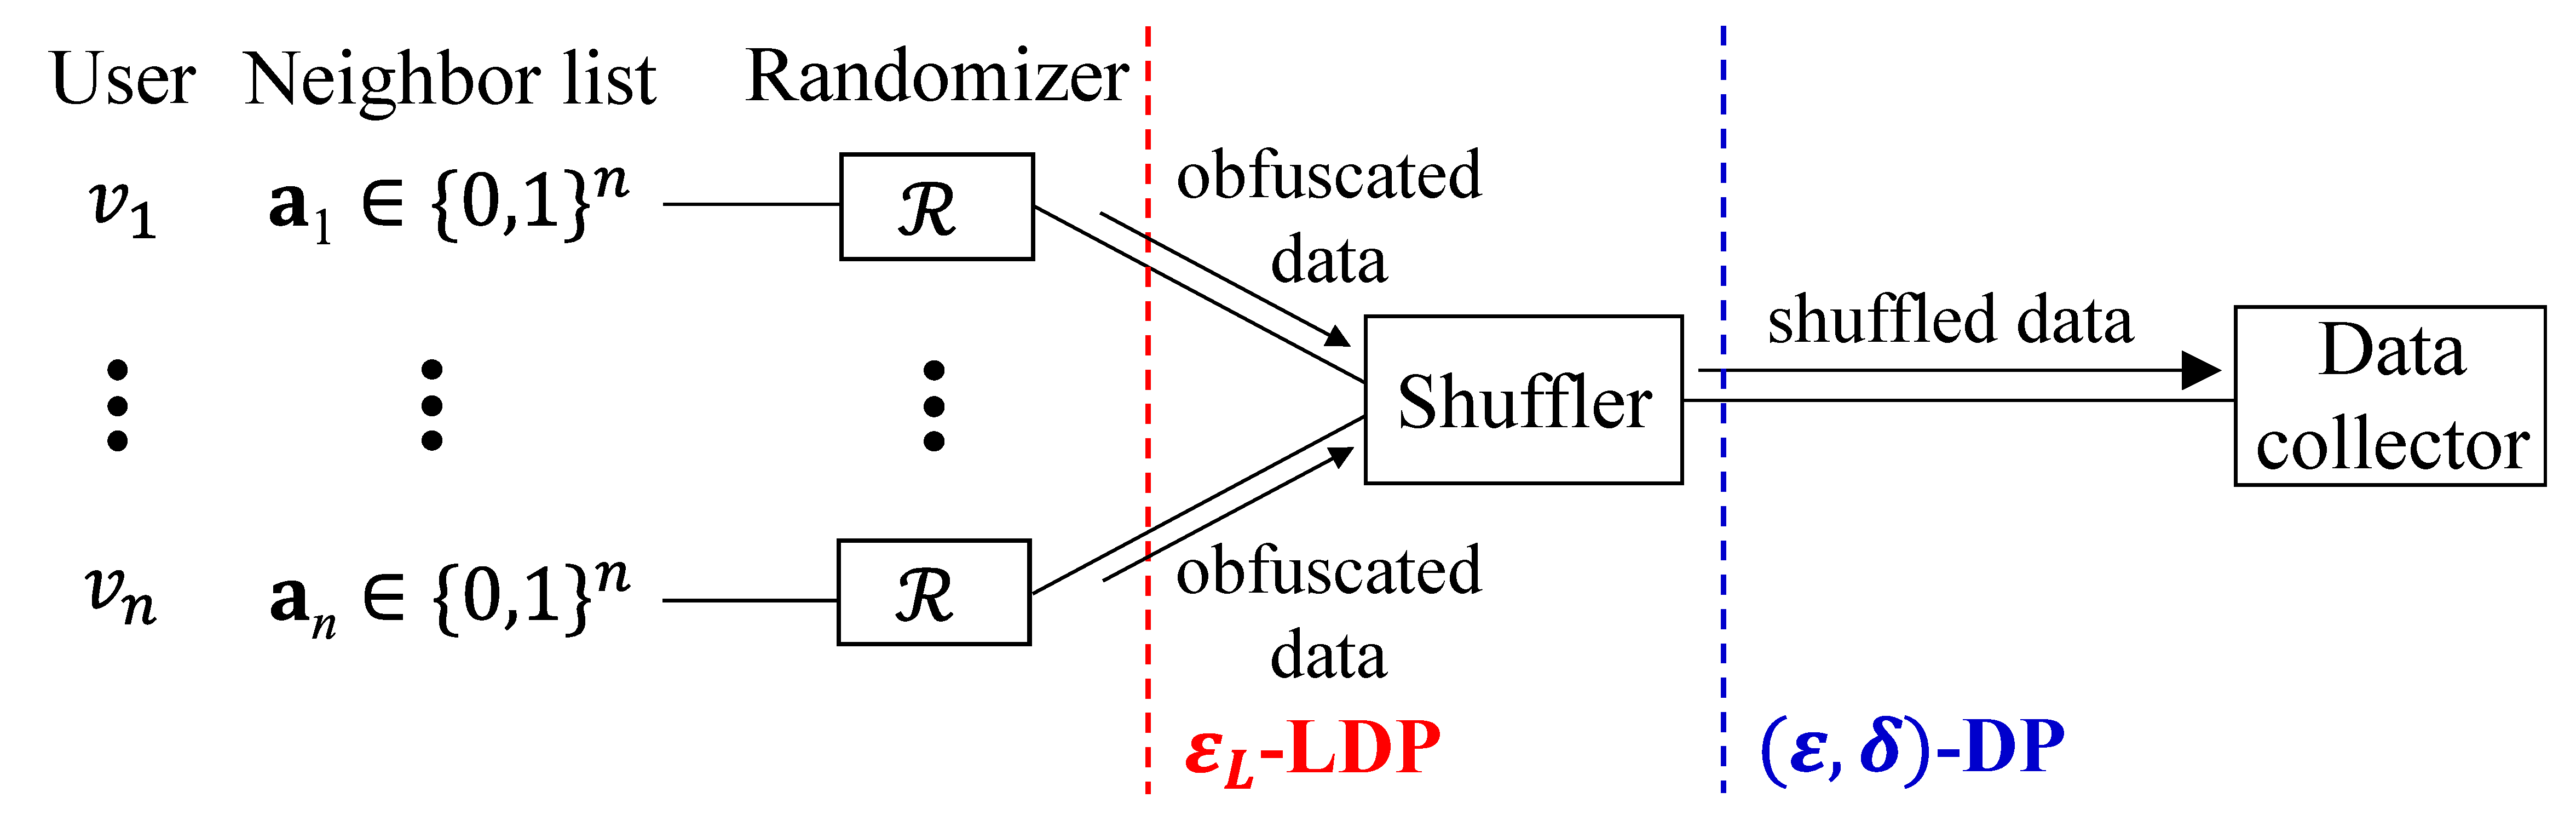
\includegraphics[width=0.99\linewidth]{fig/shuffle.pdf}
%   
%   \caption{Shuffle model. 
%   User $v_i$ obfuscates input data $x_i$ 
%   % calculated from her neighbor list $\bma_i$ 
%   and sends the obfuscated data $y_i$ to the shuffler. 
%   The shuffler sends shuffled data $y_{\pi(1)}, \ldots, y_{\pi(n)}$ to the data collector.
%   }
%   \label{chap3-fig:shuffle_model}
% \end{figure}
% Figure~\ref{chap3-fig:shuffle_model} shows the shuffle model assumed in this paper. 
Thanks to the shuffling, the shuffled data $y_{\pi(1)}, \ldots, y_{\pi(n)}$ available to the data collector provides $(\epsilon, \delta)$-DP, where $\epsilon \ll \epsilon_L$. 

Feldman \textit{et al.} \cite{Feldman_FOCS21} also propose an efficient method to numerically compute a tighter upper bound than the closed-form upper bound in Theorem~\ref{chap3-thm:shuffle}. 
We use both the closed-form and numerical upper bounds in our experiments. 
Specifically, we use the numerical upper bounds in Section~\ref{chap3-sec:experiments} and compare the numerical bound with the closed-form bound in 
\conference{the full version \cite{Imola_CCSFull22}}\arxiv{Appendix~\ref{chap3-sec:numerical_closed}}. 

Assume that $\epsilon$ and $\delta$ in (\ref{chap3-eq:shuffle_epsilon}) are constants. 
Then, by solving for $\epsilon_L$ and changing to big $O$ notation, we obtain  $\epsilon_L = \log(n) + O(1)$. 
This is consistent with the upper bound $\epsilon = O(e^{\epsilon_L / 2} / \sqrt{n})$ in \cite{Feldman_FOCS21}, from which we obtain $\epsilon_L = \log(n) + O(1)$. 
% By (\ref{chap3-eq:shuffle_epsilon}), when we treat $\epsilon$ and $\delta$ as constants, $\epsilon_L$ can be expressed as 
% $\epsilon_L = \log(n) + O(1)$. 
% Similarly, the privacy amplification bounds in \cite{Balle_CRYPTO19,Cheu_EUROCRYPT19} can also be expressed as $\epsilon_L = \Theta(\log(n))$. 
Similarly, the privacy amplification bound in \cite{Cheu_EUROCRYPT19} can also be expressed as $\epsilon_L = \log(n) + O(1)$. 
% This is smaller than other bounds, such as \cite{Balle_CRYPTO19,Erlingsson_SODA19}. 
We use the bound in \cite{Feldman_FOCS21} because it is the state-of-the-art, as described in Section~\ref{chap3-sec:related}. 
% -- it provides smaller $\epsilon$ than other bounds, such as \cite{Balle_CRYPTO19,Cheu_EUROCRYPT19,Erlingsson_SODA19}. 
%and is more general than the bound in \cite{Cheu_EUROCRYPT19} that is specific to binary RR. 
% The bound in \cite{Feldman_FOCS21} also outperforms the bound in \cite{Girgis_CCS21} when it is used without composition, which is the case with this work. 

% Note that the privacy amplification result in \cite{Feldman_FOCS21} assumes that the data elements are shuffled \textit{before} applying the local randomizers, i.e., shuffle-then-randomize. 
% However, 
% shuffling outputs of the same local randomizers (randomize-then-shuffle) 
% is equivalent to first shuffling input data and then applying the local randomizers (shuffle-then-randomize) as described in \cite{Erlingsson_SODA19}. 
% Thus, if all users adopt the same local randomizer, the result in \cite{Feldman_FOCS21} can be applied to the randomize-then-shuffle model, which gives Theorem~\ref{chap3-thm:shuffle}. 

\subsection{Utility Metrics}
\label{chap3-sub:utility}
% Following the existing work, 
We use 
the MSE (Mean Squared Error) 
% the expectation of the $l_2$ loss \cite{Kairouz_ICML16,Murakami_USENIX19,Wang_USENIX17} 
in our theoretical analysis and the relative error 
% \cite{Bindschaedler_SP16,Chen_CCS12,Xiao_SIGMOD11} 
in our experiments. 
The MSE is the expectation of the squared error 
% The $l_2$ loss is a squared error 
between a true value and its estimate. 
Let $f: \calG \rightarrow \nnints$ be a subgraph count function that can be instantiated by $f^\triangle$ or $f^\square$. 
Let $\hf: \calG \rightarrow \reals$ be the corresponding estimator. 
Let 
$\MSE: \reals \rightarrow \nnreals$ be the MSE function, which maps the estimate $\hf(G)$ to the MSE. 
% $l_2^2: \nnints \times \reals \rightarrow \nnreals$ be the expected $l_2$ loss function, which maps the true count $f(G)$ and the estimate $\hf(G)$ to the expected $l_2$ loss. 
Then the MSE can be expressed as $\MSE(\hf(G)) = \E[(f(G) - \hf(G))^2]$, 
% Then it can be expressed as $l_2^2(f(G), \hf(G)) = \E[(f(G) - \hf(G))^2]$, 
where the expectation is taken over the randomness in the estimator $\hf$. 
By the bias-variance decomposition \cite{mlpp}, 
the MSE can be expressed as a summation of the squared bias $(\E[\hf(G)] - f(G))^2$ and the variance $\V[\hf(G)] = \E[(\hf(G) - \E[\hf(G)])]^2$. 
Thus, for an unbiased estimator $\hf$ satisfying $\E[\hf(G)] = f(G)$, the MSE is equal to the variance, i.e., $\MSE(\hf(G)) = \V[\hf(G)]$. 

Although the MSE is suitable for theoretical analysis, it tends to be large when the number $n$ of users is large. 
This is because the true triangle and 4-cycle counts are very large when $n$ is large -- $f^\triangle(G) = O(n d_{max}^2)$ and $f^\square(G) = O(n d_{max}^3)$. 
Therefore, we use the relative error in our experiments. 
The relative error is an absolute error divided by the true value and is given by $\frac{|f^\triangle(G) - \hf^\triangle(G)|}{\min\{f^\triangle(G), \eta\}}$, where $\eta \in \nnreals$ is a small positive value. 
Following the convention \cite{Bindschaedler_SP16,Chen_CCS12,Xiao_SIGMOD11}, we set $\eta = \frac{n}{1000}$. 

When the relative error is well below $1$, the estimate is accurate. 
Note that the absolute error smaller than $1$ would be impossible under DP with meaningful $\epsilon$ (e.g., $\epsilon \leq 1$), as we consider counting queries. 
However, the relative error ($=$ absolute error / true count) much smaller than $1$ is possible under DP with meaningful $\epsilon$. 